%%%%%%%%%%%%%%%%%%%%%%%%%%%%%%%%%%%%%%%%%%%%%%%%%%%%%%%%%%%%%%%%%%%%%
% 
% Certains éléments de ce documents ont été repris des templates suivants :
%
%Original Source: http://www.howtotex.com
% https://tex.stackexchange.com/a/86310/10898
%http://cacr.uwaterloo.ca/~dstinson/papers/pseudocode.pdf
%
%%%%%%%%%%%%%%%%%%%%%%%%%%%%%%%%%%%%%%%%%%%%%%%%%%%%%%%%%%%%%%%%%%%%%%

\documentclass{article}
\usepackage[a4paper]{geometry}
\usepackage[myheadings]{fullpage}
\usepackage{fancyhdr}
\usepackage{lastpage}
\usepackage[T1]{fontenc}
\usepackage[utf8]{inputenc}
\usepackage{fourier}
\usepackage[protrusion=true, expansion=true]{microtype}
\usepackage[french]{babel}
\usepackage{graphicx, wrapfig, subcaption, setspace, booktabs}
\usepackage[font=small, labelfont=bf]{caption}
\usepackage{sectsty}
\usepackage{url, lipsum}
\usepackage{amsmath}
\usepackage{tikz}
\usepackage{epigraph}
\usepackage{verbatim}
\usepackage{fancybox}
\usepackage{pseudocode}
\usepackage{epsfig}
\usepackage{float}
\usepackage{titlesec}
\usepackage{url}
\usepackage{longtable}
\usepackage{colortbl}

\usepackage{subscript}

\expandafter\def\expandafter\UrlBreaks\expandafter{\UrlBreaks
  \do\*\do\-\do\~\do\'\do\"\do\_} %URL breaklines


\newcommand{\ptitre}[1]{\vspace{0.3 cm}• \textbf{#1 :}} % \ptitre{titre}
\renewcommand\epigraphflush{flushright}
\renewcommand\epigraphsize{\normalsize}
\setlength\epigraphwidth{0.7\textwidth}

\definecolor{titlepagecolor}{rgb}{0,1.0,0.3}

\newcommand\titlepagedecoration{%
\begin{tikzpicture}[remember picture,overlay,shorten >= -10pt]

\coordinate (aux1) at ([yshift=-15pt]current page.north east);
\coordinate (aux2) at ([yshift=-410pt]current page.north east);
\coordinate (aux3) at ([xshift=-4.5cm]current page.north east);
\coordinate (aux4) at ([yshift=-150pt]current page.north east);
\coordinate (aux5) at ([yshift=-550pt]current page.north east);


\begin{scope}[titlepagecolor!40,line width=12pt,rounded corners=12pt]
\draw
  (aux1) -- coordinate (a)
  ++(225:5) --
  ++(-45:5.1) coordinate (b);
\draw[shorten <= -10pt]
  (aux3) --
  (a) --
  (aux1);
\draw[opacity=0.6,titlepagecolor,shorten <= -10pt]
  (b) --
  ++(225:2.2) --
  ++(-45:2.2);
\end{scope}
\draw[titlepagecolor,line width=8pt,rounded corners=8pt,shorten <= -10pt]
  (aux4) --
  ++(225:0.8) --
  ++(-45:0.8);
\begin{scope}[titlepagecolor!70,line width=6pt,rounded corners=8pt]
\draw[shorten <= -10pt]
  (aux2) --
  ++(225:3) coordinate[pos=0.45] (c) --
  ++(-45:3.1);
\draw
  (aux2) --
  (c) --
  ++(135:2.5) --
  ++(45:2.5) --
  ++(-45:2.5) coordinate[pos=0.3] (d);   
\draw 
  (d) -- +(45:1);
\end{scope}
\end{tikzpicture}%
}

\newcommand{\HRule}[1]{\rule{\linewidth}{#1}}
\onehalfspacing
\setcounter{tocdepth}{5}
\setcounter{secnumdepth}{5}

%-------------------------------------------------------------------------------
% HEADER & FOOTER
%-------------------------------------------------------------------------------
\pagestyle{fancy}
\fancyhf{}
\setlength\headheight{15pt}
\fancyhead[L]{DUBOURDIEU, JOLY, MARLIER}
\fancyhead[R]{Le Graal de l'intégration}
\fancyfoot[R]{\thepage\ / \pageref{LastPage}}
%-------------------------------------------------------------------------------
% TITLE PAGE
%-------------------------------------------------------------------------------

 
\title{ \normalsize \textsc{Projet C 2017-2018}
		\\ [2.0cm]
		\HRule{0.5pt}
		\\ [1.0cm]
		\LARGE \textbf{\uppercase{Le Graal de l'intégration}}
    	\\ [1.0cm]
		\HRule{0.5pt} \\
		\LARGE \textsc{Partie 2 : Réalisation du projet}
		\HRule{2pt} 
		\\ [0.5cm]
		\normalsize \vspace*{3\baselineskip}
		}

\date{}



\author{DUBOURDIEU Lucas \\ 
	    JOLY Clément \\
		MARLIER Romain }

\begin{document}

\maketitle
\begin{figure}[b]
    \centering
    
\includegraphics[scale=0.32]{logo.png}
\end{figure}
\thispagestyle{empty}
\titlepagedecoration

\newpage

\tableofcontents
\newpage
%-------------------------------------------------------------------------------
% Section title formatting
\sectionfont{\scshape}
%-------------------------------------------------------------------------------

%-------------------------------------------------------------------------------
% Body
%-------------------------------------------------------------------------------
\section{Introduction}

Cette partie du rapport final présentera l'état de l'art des programmes de recommandations ainsi que le travail que nous avons réalisé pour mettre au point deux interfaces permettant aux utilisateurs de se voir recommander des films.

\section{État de l'art} \cite{ref1} \cite{ref2} \cite{ref4} \cite{ref5} \cite{ref6} \cite{ref7} \cite{ref8} \cite{ref9} \cite{ref10} \cite{ref12}
\subsection{Histoire}

Un système de recommandation est un moyen mis en place pour proposer un contenu spécifique à un utilisateur. Ce contenu est souvent associé aux goûts de l'utilisateur afin de faciliter les recherches de ce dernier ou de lui proposer un contenu inconnu en adéquation avec ses préférences.\\

L’essor du numérique au cours de la seconde moitié du XXème siècle a favorisé le développement de ces systèmes de recommandation. Au départ, ces principaux systèmes utilisaient le principe d’indexation (Van Rijsbergen, 1979) qui consistait à associer chaque objet à un label. Il était alors aisé de trouver le contenu associé à un label. 1989 vit la création du Web et avec lui une multitude d’algorithmes permettant de répondre aux demandes des utilisateurs, les moteurs de recherche. Néanmoins ces derniers utilisaient le fameux principe d'indexation. Avec la multiplication des sites web, la qualité du service rendu par les moteurs de recherche était médiocre, autant par sa quantité que par sa pertinence.
\\

Il fallut attendre 1992 et les travaux de  Paul Resnick et John Riedl pour voir apparaître le premier système de recommandation collaboratif. Ce système utilisait un principe simple mais fondamental de notation. L'idée principale est que l'utilisateur va associer des notes au contenu. Par exemple, si une personne A et une personne B ont mis les mêmes notes à des contenus similaires, alors il est fortement probable que la personne A aimera tout ce que la personne B a aussi aimé. On peut donc efficacement proposer des recommandations à la personne A.\\

Les années suivantes, plusieurs systèmes de recommandation se sont distingués. Ils apportaient chacun des avantages et des inconvénients, tant en ce qui concerne la pertinence des résultats que dans le temps d’exécution ou dans la place mémoire. La nuance entre les différents systèmes de recommandation réside dans la manière dont ils utilisent ces informations. Ainsi, certains se focaliseront uniquement sur les goûts de l'utilisateur tandis que d'autres compareront les goûts des utilisateurs entre eux. D'autres systèmes de recommandation ne demanderont pas explicitement l'avis de l'utilisateur mais récolteront des informations sur l'activité de ce dernier. Il est donc primordiale d'étudier et de comparer entre eux chacun de ces systèmes pour pouvoir ensuite proposer le système de recommandation le plus pertinent pour la réalisation de notre projet.

\subsection{Recommandation personnalisée et objet}
\subsubsection{Principe}

Afin de d'illustrer nos propos, nous nous placerons dans le contexte où le système de recommandation propose un contenu cinématographique à l'utilisateur.\\

La première étape d'un système de recommandation personnalisée (et même d’un système de recommandation en général) est la collecte d'informations. Ces informations sont récoltées directement auprès de l'utilisateur. Le fait de noter un film ou de laisser un commentaire est une information active, l'utilisateur exprimant explicitement ses choix. Les recherches que peut faire l'utilisateur tout comme le temps passé sur une page web sont des informations passives. Salton et Buckley ont même  soutenu en 1988 que l’absence de données peut aussi, dans une certaine mesure, permettre d'appréhender les goûts de l'utilisateur.

Les informations peuvent être mises sous forme matricielle afin de faciliter la compréhension.

\begin{longtable}[c]{lllll}& Film1 & Film2  & Film3 & Film4 \\ \cline{2-5} 
\endfirsthead
%
\endhead
%
\multicolumn{1}{l|}{Note} & \multicolumn{1}{l|}{5}   & \multicolumn{1}{l|}{2}   & \multicolumn{1}{l|}{} & \multicolumn{1}{l|}{} \\ \cline{2-5} 
\multicolumn{1}{l|}{Visionné} & \multicolumn{1}{l|}{Oui} & \multicolumn{1}{l|}{Oui} & \multicolumn{1}{l|}{Oui} & \multicolumn{1}{l|}{Non} \\ \cline{2-5} 
\multicolumn{1}{l|}{Pourcentage visionné} & \multicolumn{1}{l|}{100} & \multicolumn{1}{l|}{75}  & \multicolumn{1}{l|}{25}  & \multicolumn{1}{l|}{}    \\ \cline{2-5} 
\multicolumn{1}{l|}{Ignoré}  & \multicolumn{1}{l|}{Non} & \multicolumn{1}{l|}{Non} & \multicolumn{1}{l|}{Non} & \multicolumn{1}{l|}{Oui} \\ \cline{2-5} 

\label{my-label}\\
\end{longtable}

Une fois la collecte d'informations achevée, les systèmes de recommandation personnalisée vont les traiter. Ils utilisent alors les informations récoltées pour un utilisateur en particulier et les mettent en corrélation avec du contenu que l'utilisateur n'a pas encore vu. Ce contenu est lui même détaillé afin de pouvoir être comparé. Les films peuvent par exemple renvoyer à un réalisateur, à des acteurs ou à des genres. Encore une fois un modèle matriciel permet un représentation claire.

\begin{longtable}[c]{lllll}
 & Film1 & Film2 & Film3 & Film4 \\ \cline{2-5} 
\endhead
%
\multicolumn{1}{l|}{Auteur} & \multicolumn{1}{l|}{Nom1} & \multicolumn{1}{l|}{Nom2} & \multicolumn{1}{l|}{Nom3} & \multicolumn{1}{l|}{Nom1} \\ \cline{2-5} 
\multicolumn{1}{l|}{Policier} & \multicolumn{1}{l|}{Oui} & \multicolumn{1}{l|}{Non} & \multicolumn{1}{l|}{Non} & \multicolumn{1}{l|}{Oui} \\ \cline{2-5} 
\multicolumn{1}{l|}{Comique} & \multicolumn{1}{l|}{Non} & \multicolumn{1}{l|}{Oui} & \multicolumn{1}{l|}{Non} & \multicolumn{1}{l|}{Oui} \\ \cline{2-5} 
\multicolumn{1}{l|}{Romance} & \multicolumn{1}{l|}{Non} & \multicolumn{1}{l|}{Oui} & \multicolumn{1}{l|}{Oui} & \multicolumn{1}{l|}{Non} \\ \cline{2-5} 
\multicolumn{1}{l|}{Drama} & \multicolumn{1}{l|}{Oui} & \multicolumn{1}{l|}{Non} & \multicolumn{1}{l|}{Non} & \multicolumn{1}{l|}{Oui} \\ \cline{2-5} 
\label{my-label2}\\
\end{longtable}

Salton et Buckley ont proposé en 1988 de pondérer les caractéristiques de chaque contenu. Ainsi certaines caractéristiques sont jugées plus importantes que d'autres. Ces pondérations proviennent d'une approche subjective de la personne qui met au point le système de recommandation. On peut donc penser qu'un utilisateur privilégiera davantage le genre d'un film qu'un acteur en particulier.

Un autre célèbre système de recommandation est la méthode de retour de pertinence de Rocchio. Il permet à l'utilisateur de juger lui même si les recommandations qui lui sont faites sont pertinentes. Ainsi cette méthode prendra en compte l'avis de l'utilisateur pour adapter ses recommandations.


\subsubsection{Exemples}

- L'un des projets pionniers en matière de recommandation individuelle a été INFOSCOPE (Fischer and Stevens, 1991). Ce système permettait la création de groupes de discussion qui correspondraient au profil des utilisateurs. Ce système se décompose en quatre étapes~:
\begin{itemize}
    \item L'interaction de l'utilisateur avec les groupes de discussion existants
    \item L'utilisateur aime un groupe s'il lit un certain nombre de messages de ce dernier.
    \item Lorsque la base de donnée est suffisamment importante l'utilisateur se voit proposer des groupes
    \item Si un groupe recommandé ne lui plaît pas, il peut le signaler et le système s'adaptera.
\end{itemize}

\begin{itemize}
\item Les annonces publicitaires d'internet (Goolge, Facebook,...) utilisent les actions actives et passives de l'utilisateur. Se sont des sytèmes de recommandation personnaliés

\item Certaines structures multimédia utilisent des facettes de la recommandation personnalisée. Cette utilisation n'est cependant jamais le coeur du système de recommandation de ces sites.
\end{itemize}

\subsubsection{Synthèse}
Les systèmes de recommandation personnalisée ont l'avantage de proposer des résultats pertinents qui ne demande pas aux systèmes de connaître les particularité du contenu qu'ils traitent. Ils ont cependant besoin de récolter des informations auprès de l'utilisateur. Un nouvel utilisateur ne bénéficiera donc pas de recommandations.
Les systèmes de recommandation personnalisés sont actuellement très peu utilisés, on leur préférera d'autres systèmes jugés plus pertinents et qui répondent plus facilement aux problèmes de temps et de place mémoire. 

Ils ont cependant posé les bases de tous les autres systèmes de recommandation et continuent d'être utilisés dans de rares cas.

\subsection{Recommandation coopérative}
\subsubsection{Principe}
Les systèmes de recommandation coopérative, ou coopération sociale, recueillent les préférences des utilisateur (au travers de notes par exemples) et corrèlent les goûts des utilisateurs entre eux. L'idée centrale de ces systèmes est que si deux personnes aiment le même contenu dans le passé, elles aimeront le même dans le future.
Il existe deux différents type de recommandation sociale :

\begin{itemize}
    \item memory-based
    \item model-based
\end{itemize}

La recommandation coopérative utilise la notions de \textbf{profils utilisateur}.
Un profil utilisateur correspond à une entité censée représenter un ensemble d'individus ayant les mêmes goûts. Ainsi le système de recommandation associe chaque utilisateur à un profit utilisateur. Dès lors le système proposera les mêmes films à tous ceux associés à ce profil. Cette méthode a pour avantage de ne pas nécessiter de connaissances précises sur le contenu traité, mais uniquement sur les goûts et la personnalités des utilisateurs.

\subsubsection{Les différentes méthodes de recommandation coopérative}
\paragraph{La méthode memory-based}

La méthode memory-based compare les notes (ou préférences) des utilisateurs entre eux. Pour cela les notes de chaque utilisateur vont tout d'abord être stockées comme dans le modèle ci-dessous~:


\begin{longtable}[c]{lcccc}
     & \multicolumn{1}{l}{Film1} & \multicolumn{1}{l}{Film2} & \multicolumn{1}{l}{Film3} & \multicolumn{1}{l}{Film4} \\ \cline{2-5} 
\endhead
%
\multicolumn{1}{l|}{Utilisateur1} & \multicolumn{1}{c|}{5}    & \multicolumn{1}{c|}{}     & \multicolumn{1}{c|}{2}    & \multicolumn{1}{c|}{4}    \\ \cline{2-5} 
\multicolumn{1}{l|}{Utilisateur2} & \multicolumn{1}{c|}{2}    & \multicolumn{1}{c|}{4}    & \multicolumn{1}{c|}{4}    & \multicolumn{1}{c|}{2}    \\ \cline{2-5} 
\multicolumn{1}{l|}{Utilisateur3} & \multicolumn{1}{c|}{2}    & \multicolumn{1}{c|}{4}    & \multicolumn{1}{c|}{}     & \multicolumn{1}{c|}{1}    \\ \cline{2-5} 
\multicolumn{1}{l|}{Utilisateur4} & \multicolumn{1}{c|}{4}    & \multicolumn{1}{c|}{2}  & \multicolumn{1}{c|}{}     & \multicolumn{1}{c|}{5}    \\ \cline{2-5} 
\multicolumn{1}{l|}{Utilisateur5} & \multicolumn{1}{c|}{2}    & \multicolumn{1}{c|}{2}    & \multicolumn{1}{c|}{2}    & \multicolumn{1}{c|}{}     \\ \cline{2-5} 

\label{my-label3}\\
\end{longtable}

Si l'on cherche à savoir si l'utilisateur 4 peut aimer le film 3, le système va faire une moyenne pondérée avec les différentes notes des autres utilisateurs. Cette pondération provient de la corrélation des goûts entre les différents individus.
Deux méthodes de pondérations sont actuellement largement utilisées~:

\emph{Soit Vij la note donnée à l'utilisateur i pour le film j (Vij = ? si l'utilisateur n'a pas noté le film). Soit Uij la corrélation entre les utilisateurs i et j.}
\begin{itemize}
    \item Le coefficient de corrélation de Pearson renvoie un résultat entre -1 et 1. Plus le résultat est proche de 1, plus la corrélation entre les utilisateurs i et k sera importante. Le coefficient de corrélation de Pearson se calcule de la manière suivante :
    \begin{equation}
        U_{ij} = \frac{\sum_{k=0} ^m (V_{ik}-V_{i})(V_{jk}-V_{j})}{\sqrt{\sum_{k=0}^m (V_{ik}-V_{i})^2 \sum_{k=0}^m (V_{jk}-V_{j})^2 }}
    \end{equation}
    
    \item La similarité par cosinus renvoie elle aussi un coefficient entre -1 et 1. Son expression est la suivante :
    \begin{equation}
        U_{ij} = \cos(Ui, Uj)= \frac{\sum_{k=1}^m V_{ik}V_{jk}}{\sqrt{\sum_{k=1}^m V_{ik}^2 \sum_{k=1}^m V_{jk}^2}}
    \end{equation}
    \emph{Il est à noter que bien que moins utilisé, d'autres coefficient de corrélation existent, telle que la corrélation de Ringo ou le coefficient de corrélation de Spearman.}
\end{itemize}

La note théorique que l'utilisateur va donner à un film k qu'il n'a pas vu est alors estimée par la formule :
\begin{equation}
    V_{ik}^*=K \sum_{V_{jk}\neq ?} U_{kj} V_{jk}
\end{equation}


\textbf{L'exemple ci-dessous provient d'un article Steeve Huang publié sur Hackernoon.} \\

Le système de recommandation va au départ calculer la similarité entre l'utilisateur E et les autres individus. L'expression \textbf{NA} signifie que les utilisateurs n'ont pas assez de films en commun pour être comparés.


\begin{figure}[h]
    \centering
    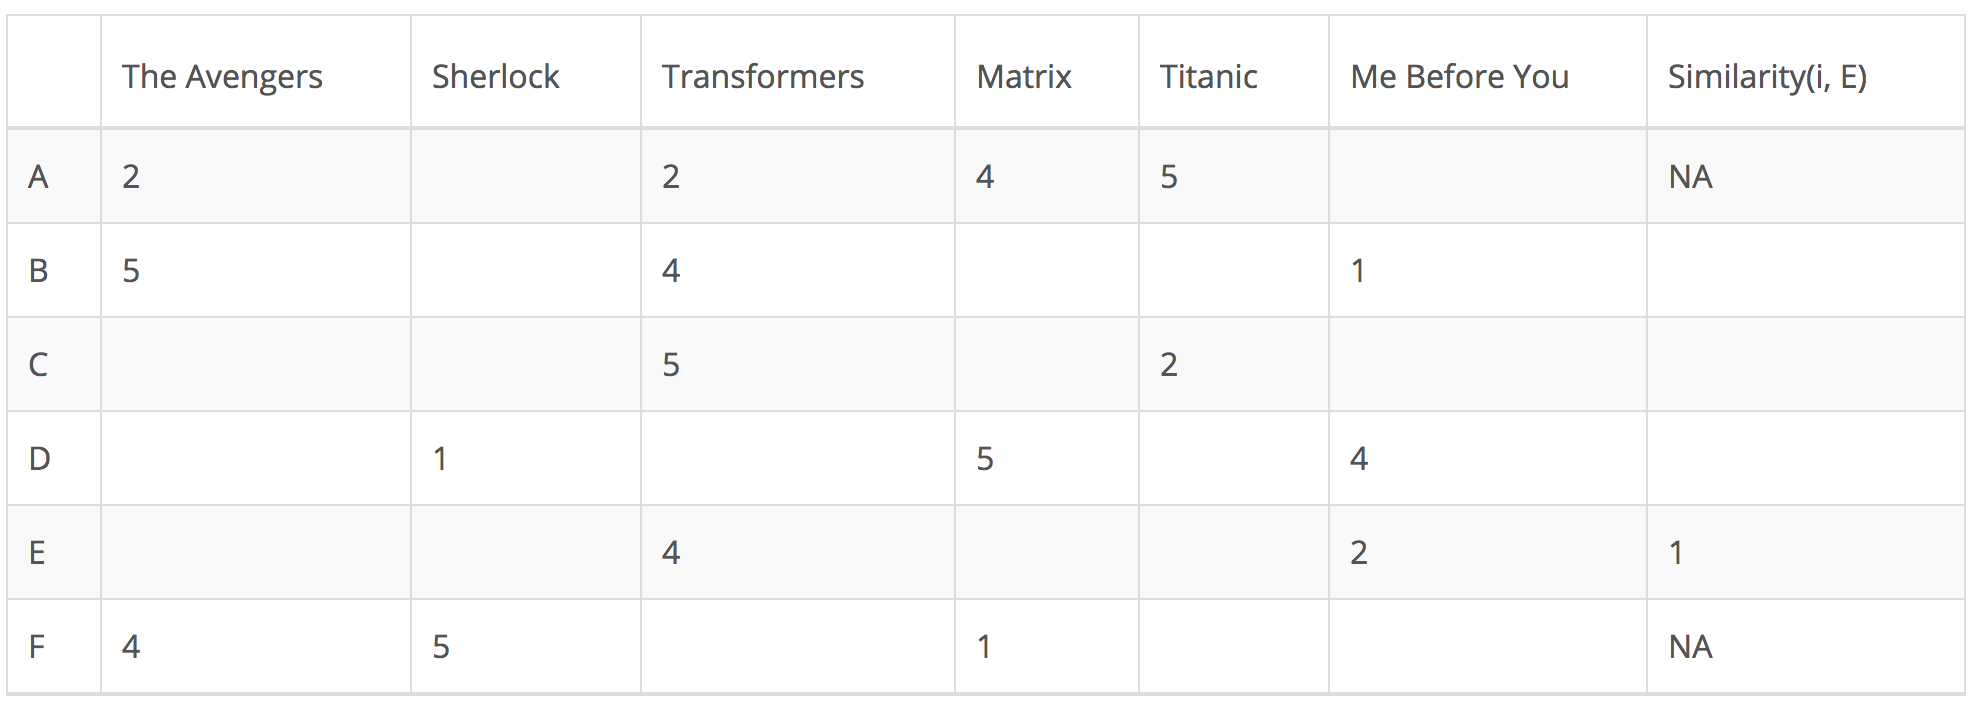
\includegraphics[scale=0.17]{Images/tab.png}
\end{figure}

L'étape suivante est de calculer une note estimative pour les films que l'utilisateur E n'a pas encore visionné.

\begin{figure}[h]
    \centering
    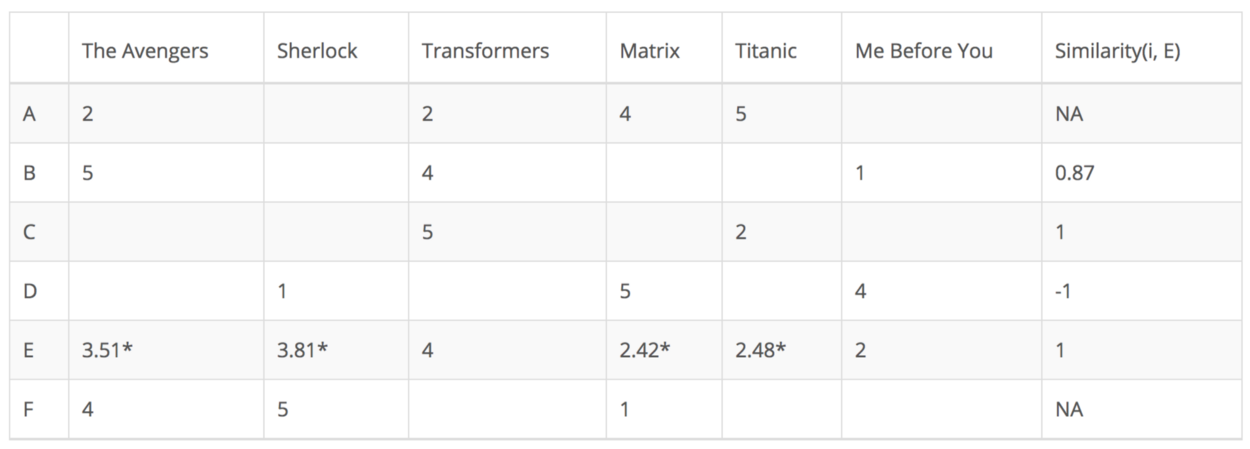
\includegraphics[scale=0.29]{Images/tab2.png}
\end{figure}

Le principal problème rencontré par cette méthode apparaît lorsqu'il faut traiter des millions d'individus. La méthode des "meilleurs voisins" répond à cette problématique. Elle consiste à sélectionner les individus ayant la plus forte corrélation avec l'utilisateur étudié. Un seuil peut tout simplement être choisi afin de délimiter les utilisateurs "proches" des utilisateurs "éloignés". Afin d'obtenir les résultats les plus probants, plusieurs études ont montré que le nombre de "meilleurs voisins" est optimal lorsqu'il se situe entre 20 et 50.

\paragraph{La méthode model-based}

Contrairement à la méthode \textbf{memory-based} qui compare les utilisateurs entre eux, la méthode \textbf{model-based} compare le contenu. Cette méthode établie dans notre exemple un coefficient de corrélation entre les différents films. La formule de similarité par cosinus (définie ci-dessus) est largement employée pour cette méthode.


La méthode \textbf{model-based} permet d'éviter les problèmes mémoires de la méthode \textbf{memory-based}. \\

\textbf{En poursuivant l'exemple de l'article de Steeve Huang publié sur Hackernoon.}\\

Dans le cas où l'on souhaiterai estimer les notes que pourrait avoir \emph{Me Before You}, le tableau précédent se remplirait comme ci-dessous :

\begin{figure}[h]
    \centering
    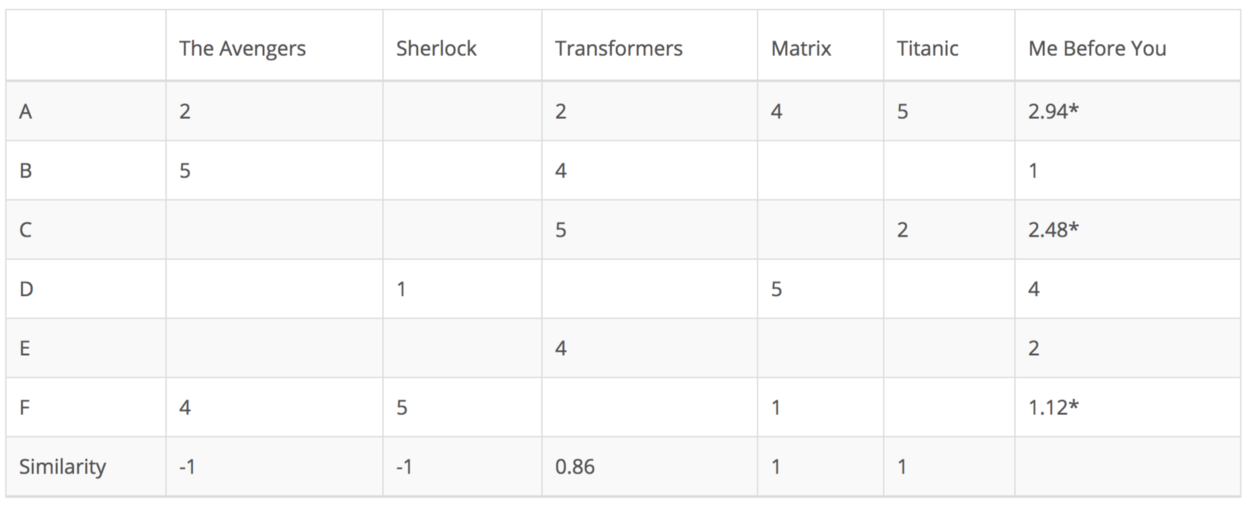
\includegraphics[scale=0.27]{Images/tab3.png}
\end{figure}

Si la méthode précédente remplissait notre tableau ligne par ligne (utilisateur par utilisateur), le \textbf{model-based} rempli le tableau colonne par colonne (film par film).

\subsubsection{Synthèse}

Les systèmes de recommandation sociale étudient les comportements des masses afin d'estimer les préférences des individus. Les profils d'utilisateurs permettent ainsi aux recommandations d'être plus satisfaisante que celles des systèmes de recommandation personnelle. Les résultats probant ainsi que l'adaptabilité de ces méthodes sur les différentes plates-formes ont permis aux systèmes de recommandation sociale de se développer considérablement.


Certains problèmes persistent néanmoins. Un nombre trop important d'utilisateurs peut entraîner des problèmes de mémoire. Les nouveaux utilisateurs auront une recommandation peut fiable et il est peu probable que tout le contenu soit noté. De plus, le système de note dépend des utilisateurs, or sur une grande quantité d'utilisateurs, seul une minorité note régulièrement le contenu qu'ils apprécient (ou déprécient).


\subsection{Recommandation dite “Hybride”}

La recommandation hybride est un mélange des recommandations présentées précédemment. De part leur efficacité, les systèmes de recommandation hybride sont les systèmes de recommandation les plus utilisés. Ils permettent de pallier les problèmes des précédents systèmes de recommandation, à savoir la recommandation d'un objet vu par peu d'utilisateurs (problème de rareté), la recommandation pour les nouveaux utilisateurs ainsi que le cas où deux personnes auraient les mêmes goûts mais vu des films différents. Dans ce dernier cas les algorithmes précédent ne permettaient pas de mettre en corrélation les préférences de ces deux utilisateurs.

Les systèmes de recommandation hybrides vont donc utiliser la recommandation objet et la recommandation sociale. Ils vont ensuite combiner ces recommandations au moyen de pondération, corrélation...

\subsubsection{Exemples}

La recommandation hybride est largement utilisée par les géants de l'industrie, tels que Google, Netflix, Amazon...\\

Amazon combine parfaitement les différents systèmes de recommandation. Grâce à ses propositions basées sur "les autres utilisateurs ont aussi aimé ceci~:", Amazon a réalisé 30\% de son chiffre d'affaire en 2009. Amazon propose aussi des produits en se basant sur le comportement de l'utilisateur (page consultée, produits achetés,...)\\

Google est passé maître dans l'art d'utiliser les différents aspects des systèmes de recommandation. Proposant les sites les plus consultés, les saisies automatiques en se basant sur l'historique de l'utilisateur ou bien en corrigeant les requêtes qu'il juge erronées, l'algorithme de Google est en perpétuelle amélioration afin de répondre au mieux aux demandes des utilisateurs.\\

Géant du monde cinématographique, Netflix mélange lui aussi les différentes facettes des systèmes de recommandation. Il utilise autant les films regardés que le profil d'utilisateur pour fournir des recommandations. De plus, entre 2006 et 2009 un concours a été organisé par Netflix, le Netflix Prize, afin d'améliorer leur algorithme. Le vainqueur de ce concours pouvant gagner 1 000 000 \$.


\label{sec:orgda54585}
\section{Recommandation à base de filtrage collaboratif :}
\label{sec:orgc28a1b4}


Des exemples du fonctionnement du programme exposé ici se trouve en fin de partie.

\subsection{Introduction :}
\label{sec:orgfb9f7bf}

Nous avons retenu et implanté une solution de recommandation par filtrage
collaboratif. On construit donc une matrice à base des préférences
utilisateurs, selon la méthode \emph{memory-based} exposée dans l’état de l’art :
chaque colonne de la matrice regroupe les notes attribuées par les utilisateurs,
qui sont eux sur les lignes. L’absence de note est marquée par un 0 et ces
notes sont comprises entre 0 et 5.

Il s’agit ensuite de compléter ces zéros par factorisation
approximative. On cherche à obtenir deux matrices P et Q telles que le produit
matriciel de P et de Q soit environ égale à la matrice R. Cet égalité
approximative est considérée au sens de la différence coefficient à coefficient
(pour les coefficients non nuls) entre le produit $PQ$ et la matrice $R$ originale.
Les coefficients nuls de la matrice R sont par contre non-nuls dans $PQ$ et on
interprète le nombre obtenu comme la note qu’aurait attribué l’utilisateur au
film. On déduit finalement de cette note hypothétique les recommandations.

En notant \textit{m} et \textit{n} respectivement le nombre de lignes et de colonnes
(respectivement) de $R$, la matrice $P$ est de taille $m \times k$ et $Q$, de taille
$k \times n$. La constante k est le nombre de facteurs sous-jacent à la notation des
films, autrement dit le nombre de critères que les utilisateurs ont retenu pour
attribuer une note à un film. On postule son existence et sa valeur pour faire
fonctionner l’algorithme.

Pour finir, je me suis basé sur l’algorithme exposé dans l’article de Albert Au Yeung, \textbf{Matrix Factorization : A Simple Tutorial and Implementation in Python} \cite{ref13}.
Cet algorithme commence par générer aléatoirement $P$ et $Q$, puis il « manipule »
les coefficients de ces matrices pour que le produit approche de R de plus en
plus finement. Il s’agit d’une \emph{minimisation d’erreur}.

\subsection{Implantation :}
\label{sec:orgc4e9e35}
\begin{enumerate}
\item Fichiers sources et bibliothèque utilisée :
\label{sec:org92d7f0a}

L’algorithme a principalement été implanté dans le fichier \texttt{factorisation.c}.
Les tests résident dans le fichier \texttt{factorisation\_test.c}.

Un fichier \texttt{factorisation.h} décrit les fonctions destinées à être utilisées
dans le reste du programme. On fournit ainsi à l’utilisateur une fonction
auxiliaire, qui alloue les matrices $P$ et $Q$, avec la taille adéquate. Ces
matrices sont placées dans une structure, avec la matrice $R$. La fonction qui
factorise à proprement parler prend cette structure en paramètre et modifie en
place les matrices $P$ et $Q$. Charge ensuite au reste du programme de libérer ces
matrices après utilisation.

La bibliothèque retenue est GSL, \emph{Gnu Scientific Library}. Elle permet la
manipulation de matrice, génère des nombres aléatoires, fournit des fonctions
mathématiques…

Elle est complétée par quelques utilitaires écrit par nos soins, dans le fichier
\texttt{tools.h}. Par exemple, une de ces fonctions auxiliaire affiche une matrice
d’une manière compréhensible par un être humain.

\item Optimisations :
\label{sec:org0bdbaff}
Cette partie de factorisation de matrice est cruciale pour le projet et les
résultats des recommandations doivent pouvoir être obtenus rapidement. Le code
correspondant a donc été l’objet d’une attention particulière.
\begin{enumerate}
\item Choix des paramètres :
\label{sec:org401be5e}
\begin{enumerate}
\item Nombre de critères sous-jacents (k) :
\label{sec:orgc72a232}
Le nombre de critères sous-jacents est déterminé empiriquement, par des tests.
Comme décrit plus loin, il ne doit pas être trop faible, pour la stabilité
numérique de l’algorithme.

Quand on augmente k, on accroît le temps de calcul et la pertinence des
suggestions. Celles-ci sont moins souvent aberrantes, on obtient peu ou plus de
notes négatives ou supérieures à 5.
\item Vitesse d’approche (\(\alpha\)) et coefficient de régularisation (\(\beta\)) :
\label{sec:org9db6c37}
Le paramètre \(\alpha\) permet de régler la \emph{vitesse} à laquelle on s’approche de
l’erreur minimale. S’il est trop grand, on risque de ne pas trouver le
minimum ou de ne pas s’en approcher assez. S’il est trop faible, on
augmente inutilement la durée des calculs.

Le \emph{coefficient de régularisation} \(\beta\) permet de conserver des valeurs comprises
entre 0 et 5. Il évite ainsi des notes aberrantes (négatives ou supérieures à
5).

Pour ces deux paramètres, nous avons expérimenté différentes valeur pour
comprendre leur influence, puis nous avons utilisé les valeurs indiquées dans la
littérature.
\end{enumerate}
\item Limitation du nombre de copies :
\label{sec:org4675e5e}
Une attention particulière a été prêtée à la limitation du nombre de copies de
données, afin d’améliorer les performances. Les pointeurs du langage C ont donc
étés abondamment utilisés.

De plus, une structure de données a été créée pour regrouper les pointeurs vers
les coefficients et la majorité des résultats. Un pointeur vers cette structure
est ensuite passé de fonction en fonction, limitant les calculs superflus et les
copies de valeur.
\end{enumerate}

\item Problèmes rencontrés :
\label{sec:orgee5739d}

Étant donné, d’une part, notre faible expérience avec le langage C, assurément renforcée par
ce projet, et, d’autre part, la relative complexité de ce code, un temps
considérable (environ 20 heures pour cette partie) a été employé pour chasser
les bugs.

Ce temps doit toutefois être relativisé, puisqu’il a aussi été mis à profit pour
approfondir notre maîtrise de l’outil gdb.

Au-delà des petites erreurs vite débusquées, un problème mérite d’être exposé ici.

\begin{enumerate}
\item Inf \& NaN :
\label{sec:org80d2de1}

Pour des paramètres k petits, les matrices P et Q se remplissent de \emph{Not a Number},
\textbf{NaN}. Comme vu en cours de Mathématiques Numériques, ceci survient lors de
certaines opérations irréalisables dans l’ensemble des réels. Par exemple, le
calcul de racine de -1 ou une division de l’infini, \textbf{inf} par l’infini renvoient
NaN.

Le code itérant à de multiples reprises sur l’ensemble de la matrice,
l’utilisation de point d’arrêt conditionnels et point d’arrêt à la
lecture/écriture de variable dans gdb a permis de cerner l’erreur mais c’est
avérée laborieuse et imprécise malgré tout.

L’utilisation de la bibliothèque \texttt{fenv} (bibliothèque standard C99) a été
décisive. Il a été possible de demander l’interruption du programme à la
première erreur de représentation à virgule flottante (inf ou NaN). Le
processeur lève une exception, qui est ensuite remonté au noyau qui envoie un
signal \texttt{SIGFPE} au programme. L’exécution de celui-ci est interrompue.

L’outil gdb est capable de se placer dans l’environnement du programme au moment
de l’interruption. On peut donc déterminer précisément l’opération responsable
du problème. Dans le cas qui nous occupe, on multipliait deux nombres trop
grands pour que le résultats puisse être stocké dans un double.

Après investigation, nous nous sommes aperçu qu’un des produits scalaires
tendait à croître démesurément, entraînant le dépassement.

\begin{enumerate}
\item Solutions :
\label{sec:org966338a}

Une fois le problème précisément identifié, plusieurs solutions ont été envisagées.

Les nombres sont pour l’essentiel encodés en \texttt{double}. Il a été envisagé de
passer en \texttt{long double}, pour bénéficier de la possibilité de représenter des
nombres plus grands. Cependant, cela n’aurait fait que repousser les limites au
sein des quels nous pouvions opérer, sans résoudre le problème.

Nous observons cependant que les NaN n’apparaissent que pour des calculs où k est
relativement petit devant m et n. Nous sommes finalement parvenus à la
conclusion que ce problème était la manifestation d’une limitation de
l’algorithme.

Nous avons donc pris la décision de prendre un nombre k de critères sous-jacents
plus grand, ce qui résoud le problème, au prix d’un temps de calcul accru. Une
petite amélioration de performance a été obtenue en interrompant les calculs
aussitôt que les NaN apparaissent, plutôt que de continuer à tenter de construire P et Q.
\end{enumerate}
\end{enumerate}
\end{enumerate}

\subsection{Limites de l’algorithme :}
\label{sec:org3285ae0}
Le problème évoqué précédemment nous amène à évoquer les limites de l’algorithme.
\begin{enumerate}
\item Génération des recommandations :
\label{sec:orgad7243e}

Une première limite se dégage en termes de temps de calcul initial.

Rappelons que la matrice R contient autant de lignes que d’utilisateurs, et
autant de colonnes que de films. Or, plus la base de donnée est fournie, plus
les recommandations sont pertinentes. Il est donc opportun de considérer le cas
d’une matrice R avec plusieurs dizaines de milliers de lignes et colonnes.

Dans ce contexte, la complexité en \(O(n*m*k)\) se traduit par des temps de calcul
importants. Cette faiblesse du procédé exposé ici doit toutefois être
relativisé dans la mesure où l’on obtient d’un seul coup les recommandations
pour l’ensemble des utilisateurs. Il ne faut donc refaire les calculs que pour
actualiser les recommandations.

\item Mise à jour des recommandations :
\label{sec:orgd9ed3c8}

Une deuxième limite est liée à la difficulté de mise à jour. Avec ce qui a été
 vu ici, il est impossible de mettre à jour la matrice sans reprendre l’ensemble
 des calculs. Cet aspect rend difficile la mise à jour fréquente des
 recommandations. On ne peut donc pas adapter les recommandations proposées aux
 dernières notes ajoutés par les utilisateurs.
\end{enumerate}
\subsection{Exemples :}
\label{sec:org42b0a50}
\begin{enumerate}
\item Fonctionnement général :
\label{sec:org0106ff2}
On fait fonctionner l’algorithme exposé précédement sur la matrice R (de taille
9 lignes et 8 colonnes) suivante, avec un nombre k de critères sous-jacents pris
égal à 5.

\begin{verbatim}
Factorisation d’une matrice (k=5, size1=9, size2=8)
R
[
[ 0.000, 	1.000, 	2.000, 	0.000, 	0.000, 	0.000, 	1.000, 	0.000	 ],
[ 4.000, 	0.000, 	0.000, 	2.000, 	0.000, 	4.000, 	0.000, 	1.000	 ],
[ 0.000, 	1.000, 	0.000, 	1.000, 	0.000, 	3.000, 	2.000, 	4.000	 ],
[ 0.000, 	0.000, 	0.000, 	0.000, 	2.000, 	0.000, 	4.000, 	0.000	 ],
[ 0.000, 	3.000, 	4.000, 	2.000, 	0.000, 	1.000, 	0.000, 	0.000	 ],
[ 4.000, 	0.000, 	0.000, 	4.000, 	0.000, 	2.000, 	3.000, 	0.000	 ],
[ 0.000, 	0.000, 	0.000, 	1.000, 	0.000, 	0.000, 	1.000, 	0.000	 ],
[ 0.000, 	0.000, 	1.000, 	0.000, 	0.000, 	0.000, 	0.000, 	2.000	 ],
[ 1.000, 	0.000, 	1.000, 	4.000, 	0.000, 	2.000, 	0.000, 	0.000	 ]
]
\end{verbatim}
Les matrices P et Q après génération aléatoire de leurs coefficients.
\begin{verbatim}
P
[
[ 0.346, 	0.046, 	0.613, 	0.567, 	0.498	 ],
[ 0.723, 	0.144, 	0.042, 	0.310, 	0.121	 ],
[ 0.242, 	0.381, 	0.440, 	0.599, 	0.644	 ],
[ 0.432, 	0.556, 	0.716, 	0.642, 	0.685	 ],
[ 0.096, 	0.122, 	0.057, 	0.820, 	0.125	 ],
[ 0.315, 	0.180, 	0.142, 	0.664, 	0.685	 ],
[ 0.191, 	0.436, 	0.964, 	0.868, 	0.130	 ],
[ 0.484, 	0.374, 	0.900, 	0.178, 	0.679	 ],
[ 0.622, 	0.983, 	0.440, 	0.804, 	0.994	 ]
]
Q
[
[ 0.541, 	0.255, 	0.638, 	0.575, 	0.258, 	0.191, 	0.445, 	0.149	 ],
[ 0.996, 	0.121, 	0.651, 	0.027, 	0.390, 	0.827, 	0.283, 	0.610	 ],
[ 0.236, 	0.410, 	0.677, 	0.847, 	0.649, 	0.081, 	0.120, 	0.479	 ],
[ 0.777, 	0.472, 	0.943, 	0.980, 	0.334, 	0.202, 	0.342, 	0.653	 ],
[ 0.682, 	0.609, 	0.099, 	0.766, 	0.735, 	0.241, 	0.263, 	0.960	 ]
]
\end{verbatim}

On fait ensuite fonctionner l’algorithme, pour ajuster les coefficients de
manière à ce que le produit PQ soit environ égal à R.

\begin{verbatim}
P =[
[ 0.315, 	0.236, 	0.703, 	0.532, 	-0.197	 ],
[ 1.680, 	1.206, 	-0.083, 	0.517, 	0.216	 ],
[ -0.397, 	1.539, 	0.370, 	0.401, 	0.900	 ],
[ 1.045, 	1.029, 	0.994, 	1.196, 	1.200	 ],
[ 0.249, 	0.277, 	0.471, 	1.857, 	0.066	 ],
[ 0.758, 	0.122, 	0.386, 	1.716, 	1.055	 ],
[ 0.029, 	0.277, 	0.785, 	0.595, 	-0.027	 ],
[ 0.339, 	0.292, 	0.767, 	-0.039, 	0.724	 ],
[ 0.477, 	-0.011, 	0.891, 	0.016, 	1.690	 ]
]
Q =[
[ 1.018, 	0.318, 	0.765, 	1.093, 	0.160, 	1.057, 	0.890, 	-0.569	 ],
[ 1.142, 	-0.002, 	0.609, 	-0.389, 	0.289, 	1.701, 	0.745, 	1.047	 ],
[ -0.067, 	0.291, 	0.952, 	0.892, 	0.544, 	0.249, 	0.492, 	0.933	 ],
[ 1.609, 	1.481, 	1.722, 	0.704, 	0.216, 	0.051, 	0.678, 	0.798	 ],
[ 0.331, 	0.474, 	-0.139, 	1.576, 	0.611, 	0.763, 	0.833, 	1.659	 ]
]
\end{verbatim}

Le produit PQ est à la fin du processus environ égal à R (coefficients non-nuls
peu différents).

\begin{verbatim}
R appprox = PQ
[
[ 1.336, 	1.000, 	1.999, 	0.944, 	0.496, 	0.788, 	1.000, 	0.822	 ],
[ 3.999, 	1.376, 	2.802, 	1.999, 	0.818, 	3.999, 	2.885, 	1.000	 ],
[ 2.274, 	1.000, 	1.553, 	1.000, 	1.221, 	2.999, 	2.000, 	3.999	 ],
[ 4.499, 	2.962, 	4.268, 	4.366, 	2.000, 	4.082, 	3.999, 	4.357	 ],
[ 3.552, 	2.999, 	3.999, 	2.000, 	0.820, 	1.000, 	1.976, 	2.181	 ],
[ 3.999, 	3.397, 	3.833, 	3.999, 	1.384, 	2.000, 	3.000, 	3.178	 ],
[ 1.243, 	1.106, 	1.968, 	1.000, 	0.624, 	0.708, 	1.000, 	1.435	 ],
[ 0.804, 	0.615, 	1.000, 	2.056, 	0.990, 	1.599, 	1.474, 	1.999	 ],
[ 1.000, 	1.237, 	1.000, 	3.999, 	1.595, 	1.999, 	2.275, 	3.367	 ]
]
\end{verbatim}

À titre indicatif, ceci s’exécute en quelques milisecondes.

\begin{verbatim}
Temps CPU : 0.04459 seconde(s)
\end{verbatim}
\item Paramètre k :
\label{sec:orga2db1d5}

Dans ce qui suit, on fait fonctionner l’algorithme avec les mêmes matrices R, P
et Q et on fait varier k à tout autres paramètres constants.

Matrice R choisie
\begin{verbatim}
R
[
[ 0.000, 	1.000, 	2.000, 	0.000, 	0.000, 	0.000, 	1.000, 	0.000	 ],
[ 4.000, 	0.000, 	0.000, 	2.000, 	0.000, 	4.000, 	0.000, 	1.000	 ],
[ 0.000, 	1.000, 	0.000, 	1.000, 	0.000, 	3.000, 	2.000, 	4.000	 ],
[ 0.000, 	0.000, 	0.000, 	0.000, 	2.000, 	0.000, 	4.000, 	0.000	 ],
[ 0.000, 	3.000, 	4.000, 	2.000, 	0.000, 	1.000, 	0.000, 	0.000	 ],
[ 4.000, 	0.000, 	0.000, 	4.000, 	0.000, 	2.000, 	3.000, 	0.000	 ],
[ 0.000, 	0.000, 	0.000, 	1.000, 	0.000, 	0.000, 	1.000, 	0.000	 ],
[ 0.000, 	0.000, 	1.000, 	0.000, 	0.000, 	0.000, 	0.000, 	2.000	 ],
[ 1.000, 	0.000, 	1.000, 	4.000, 	0.000, 	2.000, 	0.000, 	0.000	 ]
]
\end{verbatim}
Pour k = 3
\begin{verbatim}
Factorisation d’une matrice (k=3, size1=9, size2=8)
R appprox = PQ
[
[ 3.077, 	1.000, 	1.999, 	0.330, 	0.705, 	1.038, 	1.000, 	2.493	 ],
[ 3.999, 	-1.284, 	1.013, 	1.999, 	0.826, 	3.999, 	1.572, 	1.000	 ],
[ 6.186, 	1.000, 	3.380, 	1.000, 	1.353, 	2.999, 	2.000, 	3.999	 ],
[ 6.420, 	2.783, 	4.926, 	4.969, 	2.000, 	3.571, 	3.999, 	8.117	 ],
[ 4.412, 	2.999, 	3.999, 	2.000, 	1.331, 	0.999, 	2.315, 	6.149	 ],
[ 3.999, 	2.573, 	3.682, 	3.999, 	1.426, 	2.000, 	3.000, 	6.479	 ],
[ 1.890, 	0.937, 	1.495, 	1.000, 	0.551, 	0.753, 	0.999, 	2.300	 ],
[ 1.436, 	0.362, 	1.000, 	2.102, 	0.527, 	1.440, 	1.274, 	1.999	 ],
[ 1.000, 	0.445, 	0.999, 	3.999, 	0.657, 	1.999, 	1.987, 	2.864	 ]
]
Temps CPU : 0.03330 seconde(s)
\end{verbatim}
Pour k = 5
\begin{verbatim}
Factorisation d’une matrice (k=5, size1=9, size2=8)
R appprox = PQ
[
[ 1.336, 	1.000, 	1.999, 	0.944, 	0.496, 	0.788, 	1.000, 	0.822	 ],
[ 3.999, 	1.376, 	2.802, 	1.999, 	0.818, 	3.999, 	2.885, 	1.000	 ],
[ 2.274, 	1.000, 	1.553, 	1.000, 	1.221, 	2.999, 	2.000, 	3.999	 ],
[ 4.499, 	2.962, 	4.268, 	4.366, 	2.000, 	4.082, 	3.999, 	4.357	 ],
[ 3.552, 	2.999, 	3.999, 	2.000, 	0.820, 	1.000, 	1.976, 	2.181	 ],
[ 3.999, 	3.397, 	3.833, 	3.999, 	1.384, 	2.000, 	3.000, 	3.178	 ],
[ 1.243, 	1.106, 	1.968, 	1.000, 	0.624, 	0.708, 	1.000, 	1.435	 ],
[ 0.804, 	0.615, 	1.000, 	2.056, 	0.990, 	1.599, 	1.474, 	1.999	 ],
[ 1.000, 	1.237, 	1.000, 	3.999, 	1.595, 	1.999, 	2.275, 	3.367	 ]
]
Temps CPU : 0.04219 seconde(s)
\end{verbatim}
Pour k = 7
\begin{verbatim}
Factorisation d’une matrice (k=7, size1=9, size2=8)
R appprox = PQ
[
[ 2.311, 	1.000, 	1.999, 	0.722, 	0.734, 	1.855, 	1.000, 	1.270	 ],
[ 3.999, 	3.117, 	3.286, 	2.000, 	1.305, 	3.999, 	2.349, 	1.000	 ],
[ 3.201, 	1.000, 	2.939, 	1.000, 	1.406, 	2.999, 	2.000, 	3.999	 ],
[ 3.868, 	3.259, 	3.556, 	2.935, 	2.000, 	3.923, 	3.999, 	2.694	 ],
[ 3.476, 	2.999, 	3.999, 	2.000, 	2.100, 	1.000, 	2.068, 	1.869	 ],
[ 3.999, 	3.947, 	4.240, 	3.999, 	2.875, 	2.000, 	2.999, 	2.327	 ],
[ 0.924, 	0.691, 	1.076, 	1.000, 	0.863, 	0.407, 	0.999, 	1.472	 ],
[ 1.063, 	0.918, 	1.000, 	0.973, 	0.845, 	1.505, 	1.166, 	1.999	 ],
[ 1.000, 	2.609, 	1.000, 	3.999, 	1.969, 	1.999, 	1.979, 	1.344	 ]
]
Temps CPU : 0.05318 seconde(s)
\end{verbatim}
Les conclusions de ces observations ont été tirées dans la partie sur le choix des paramètres.
\end{enumerate}

\section{Structures de données}
Ce projet étant un projet de C et de structures de données dans cette partie nous allons étudier ces différentes structures utilisées en justifiant le choix de celles-ci en étudiant leur complexité temporelle et en mémoire ainsi que d’autres facteurs.
\subsection{Structures de données utilisées}
Les structures de données utilisées lors de ce projet sont surtout des structures linéaires à savoir des listes.
\subsubsection{Liste avec implantation contiguë }
Nous avons utilisé ce type de liste pour stocker les différents films qui composent la base de données\\
Définition des structures en C :\\
\begin{verbatim}
typedef struct movie{
    int id; //id du film
    char* title; //titre du film
    int year; //année du film
    char* director; //réalisateur du film
    string_list actors; //liste d'acteurs du film
    string_list genre; //liste de genres du film
    int duration; //durée du film
    type_movie type; //type de film (serie ou film)
    char* synopsis; //synopsis du film
    int grade; //note
}movie;

typedef struct movies{
    int max_length; //longueur de la liste
    char* user; //nom d'utilisateur
    movie** tab; //tableau contenant la liste de film
    recommendations_list recommendations; // liste d'indice des films recommandés
}movies;

\end{verbatim}

La structure movie est la structure qui permet de représenter un film elle contient donc un certain nombre d’information à savoir : 
\begin{itemize}
    \item Un id qui est utilisé pour accéder facilement au film dans la liste
    \item Le titre du film
    \item L’année de sortie
    \item Le réalisateur
    \item Le casting
    \item Les genres
    \item La durée
    \item Le type (film ou série)
    \item Le synopsis
    \item La note de l’utilisateur qui utilise l’application
\end{itemize}
\vspace{3mm}
Nous avons ensuite la structure movies qui représente le liste de film avec :
\begin{itemize}
    \item Le nombre de films
    \item Le nom de l’utilisateur utilisé dans le nom du fichier JSON le concernant
    \item Un tableau de pointeur de film
    \item La liste de recommandations de l’utilisateur
\end{itemize}
\vspace{3mm}
Ce tableau de film est donc une liste avec une implantation contiguë. Nous avons choisi cette implantation pour plusieurs raisons :
\begin{itemize}
    \item Facilité d’accès aux film l’id du film étant son indice dans le tableau nous avons donc une complexité temporelle en O(1).
    \item Comme l’id du film est aussi son indice dans le tableau nous n’avons pas de problème d’insertion étant donné que chaque id est unique.
    \item Pour ce qui est de la complexité spatiale, avec n films la fait n*taille(movie).
    \item Le nombre de film étant connu à l’avance, donné par la base de données, nous pouvons allouer la taille nécessaire sans utiliser de la mémoire inutilement.
\end{itemize}

\subsubsection{Listes chaînées}

Nous avons également utilisé des listes chaînées pour stocker la liste des acteurs et de genres il s’agit donc d’une liste chaînée de chaîne de caractère ses listes sont en général courte le problème du parcours pour accéder au ième élément n’est donc pas très important. De plus les listes d’acteurs et de genres pour différents films ne font pas toujours la même taille, avec cette implantation chaînée nous pouvons donc allouer facilement l’espace nécessaire sans connaître le nombre de genres ou d’acteurs en avance.\\
Une liste chaînée est aussi utilisée pour stocker les recommandations, voici en C les structures utilisées :


\begin{verbatim}
struct recommendations_cell{
    int id; //id du film recommandé
    double grade; //note potentiel de l'utilisateur
    struct recommendations_cell* next; //pointeur vers l'élément suivant
};
typedef struct recommendations_cell* recommendations_list;
\end{verbatim}

Dans cette liste nous avons l’id du film et la note potentiel donnée par l’utilisateur issue de l’algorithme de recommandations nous avons également un pointeur donnant l’élément suivant.\\
Cette implantation est intéressante car quand on ajoute les films recommandés dans la liste ils sont insérés de manière avoir une liste triée en fonction des notes potentiels décroissantes. Cette implantation est donc idéale pour des insertions quel que soit la position dans la liste. Lors de l’affichage des recommandations nous parcourons simplement, par exemple, les 10 premiers films de la liste.

\subsubsection{Matrice}
Une autre structure utilisée est la matrice, utilisée pour l’algorithme de factorisation c’est matrice sont exploitées avec la bibliothèque GSL

\subsection{Gestion des fichiers JSON}
Pour sauvegarder les films et les données des utilisateurs nous utilisons des fichiers JSON. Nous exploitons ces fichiers à l’aide de la bibliothèque WJElement qui permet une utilisation assez simple de ces fichiers un peu à la manière de langage objet.\\
Exemple récupération d’un attribut :\\
\begin{verbatim}
m->id = WJEInt32(elem, "movies[1].id"), WJE_GET, 0);
m->title = WJEString(elem, "movies[1].title", WJE_GET, "");
\end{verbatim}
Avec :
\begin{itemize}
    \item WJESTring, WJEInt32… en fonction du type de donnée
    \item elem qui est une structure qui représente un element dans JSON (objet, tableau…)
    \item "movies[1].id" qui est le chemin vers l’attribut que l’on veut récupérer
    \item WJE\_GET qui permet de dire que l’on souhaite accéder à cette valeur
\end{itemize}
\vspace{3mm}

De manière similaire pour affecter une valeur à un attribut :

\begin{verbatim}
    WJEInt64(elem, "movies[1]->grade", WJE_SET, grade);
\end{verbatim}
Avec :
\begin{itemize}
    \item WJE\_SET qui permet de dire que l’on souhaite affecter une valeur
    \item -	grade qui est la valeur à affecter
\end{itemize}
\subsubsection{Fichier JSON concernant la liste de films}
Ce fichier contient les informations utiles concernant les films.\\
Ce fichier est de la forme :
\begin{verbatim}
{
  "movies":[
    {
      "id": 0,
      "title": "Fast & Furious 7",
      "year": 2015,
      "director": "James Wan",
      "genres": ["Action", "Crime", "Thriller"],
      "actors": ["Vin Diesel", "Paul Walker", "Dwayne Johnson"],
      "duration": 137,
      "type": "Movie",
      "synopsis": "Deckard Shaw seeks revenge against Dominic Toretto and his family for his comatose brother."
    },

    {
      "id": 1,
      "title": "The Walking Dead",
      "year": 2010,
      "director": "",
      "genres": ["Drama", "Horror"],
      "actors": ["Andrew Lincoln", "Jon Bernthal", "Sarah Wayne Callies"],
      "duration": 44,
      "type": "Serie",
      "synopsis": "Sheriff's Deputy Rick Grimes leads a group of survivors in a world overrun by zombies."
    }
  ]
}
\end{verbatim}
\subsubsection{Les fichiers utilisateurs}
Ces fichiers contiennent les notes des films des utilisateur (0 pour les films non notés) et les 10 premiers films recommandés. Ces fichiers sont stockés dans un répertoire users afin de pouvoir scanner facilement ces fichiers. Les noms de ces fichiers sont de la forme "login\_utilisateur.json" afin d’identifier facilement l’utilisateur associé au fichier, sans lire à l’intérieur.\\
Ces fichiers sont de la forme :
\begin{verbatim}
{
    "movies":[
        {
            "id":0,
            "title":"Fast & Furious 7",
            "grade":4
        },
        {
            "id":1,
            "title":"The Walking Dead",
            "grade":0
        }
    ],
    "recommendations":[
        {
            "id":12,
            "title":"It Follows",
            "grade":4.840226e+00
        },
        {
            "id":2,
            "title":"Spectre",
            "grade":4.823346e+00
        }
    ]
}


\end{verbatim}

\section{Interfaces}
\subsection{Interface console}
L’objectif de cette partie est de faire une interface console utilisable et permettant d’avoir toutes les informations utiles concernant les films.

\subsubsection{Présentation de l'interface}

\paragraph{Connexion}
Lors du lancement du programme la première chose à faire par l’utilisateur est de saisir un identifiant. Si l’utilisateur s’est déjà connecté avec cet identifiant alors l’application va charger les notes qu’il a déjà saisies.

\paragraph{Menu principal}
Depuis ce menu l’utilisateur peut :
\begin{itemize}
    \item Noter des films en saisissant 1
    \item Consulter ses recommandations en saisissant 2
    \item Sauvegarder ses notes en saisissant 3
    \item Quitter en saisissant 4
\end{itemize}

\paragraph{Liste de films}
Quand l’utilisateur saisi 1 dans le menu pour noter les films il arrive sur la liste de films ou il peut voir les titres et la note du film. Pour sélectionner un film l’utilisateur doit rentrer le nombre devant le film

\paragraph{Détails et notation d'un film}
Une fois le film choisis, l’utilisateur peut voir les différentes informations concernant le film et il peut saisir la note entre 1 et 5, 0 pour annuler. Retour au menu automatique 

\paragraph{Recommandations}
Lorsque l’utilisateur saisi 2 sur le menu l’application va déterminer les recommandations de l’utilisateur puis afficher les 10 films recommandés sous forme de liste. L’utilisateur peut voir les détails d’un film en saisissant le nombre devant le titre du film ou il peut revenir au menu en faisant -1.

\subsection{Interface graphique}
\subsubsection{Décisions conceptuelles}

Dans le but de réaliser une interface graphique pertinente, il convient de définir correctement ce qu'est justement une interface graphique et les attentes d'un utilisateur envers cette dernière. \\
    
Définition : Un interface graphique est un outil permettant de faire le lien entre l'utilisateur et le programme au moyen de boutons, menus, pictogrammes,... \\
    
On attend donc d'une interface qu'elle soit :
\begin{itemize}
    \item intuitive
    \item facile d'utilisation
    \item agréable visuellement
\end{itemize}
    
Ces trois points ont guidé notre raisonnement afin de réaliser une interface graphique pertinente. Ils ont donc été notre ligne directrice et ont incité nos choix de conceptions. \\

La bibliothèque GTK 3.0 a été utilisé afin de réaliser l'interface graphique. Glade, qui est un outil graphique facilitant l’utilisation de GTK nous a permis de faciliter la mise en page, mise en page améliorée avec d'autres fonctions impropres à l'outil que représente Glade. \\

Après avoir étudié plusieurs sites dont la recommandation de contenu multimédia était l'activité majeur, il est apparu que notre interface devait comporter au minima ces caractéristiques :
\begin{itemize}
    \item un menu de connexion
    \item un menu permettant de naviguer entre les différents contenus
    \item une fenêtre permettant d'accéder aux informations relatives à chaque film
    \item une fenêtre permettant de voir les recommandations
    \item une fenêtre permettant de voir la bibliothèque de films
\end{itemize}



Un style graphique a été décidé au sein de l'équipe projet. Ce style graphique régira l'intégralité de l'interface. Il n'interférera pas avec les informations essentielles à l'utilisateur mais permettra de rendre l'expérience plus agréable à ses yeux.

\subsubsection{Présentation de l'interface}

\paragraph{Page de connexion}


La page de connexion de l'interface se veut sobre mais efficace. Elle offre le choix à l'utilisateur de se connecter ou de créer un nouveau compte le cas échéant. À l'instar de l'interface en ligne de commande, le programme vérifiera si l'utilisateur est répertorié parmi les utilisateurs existants. Un fichier JSON vierge contenant ses données sera créé s'il s'agit d'un nouvel utilisateur.

\begin{figure}[H]
    \centering
    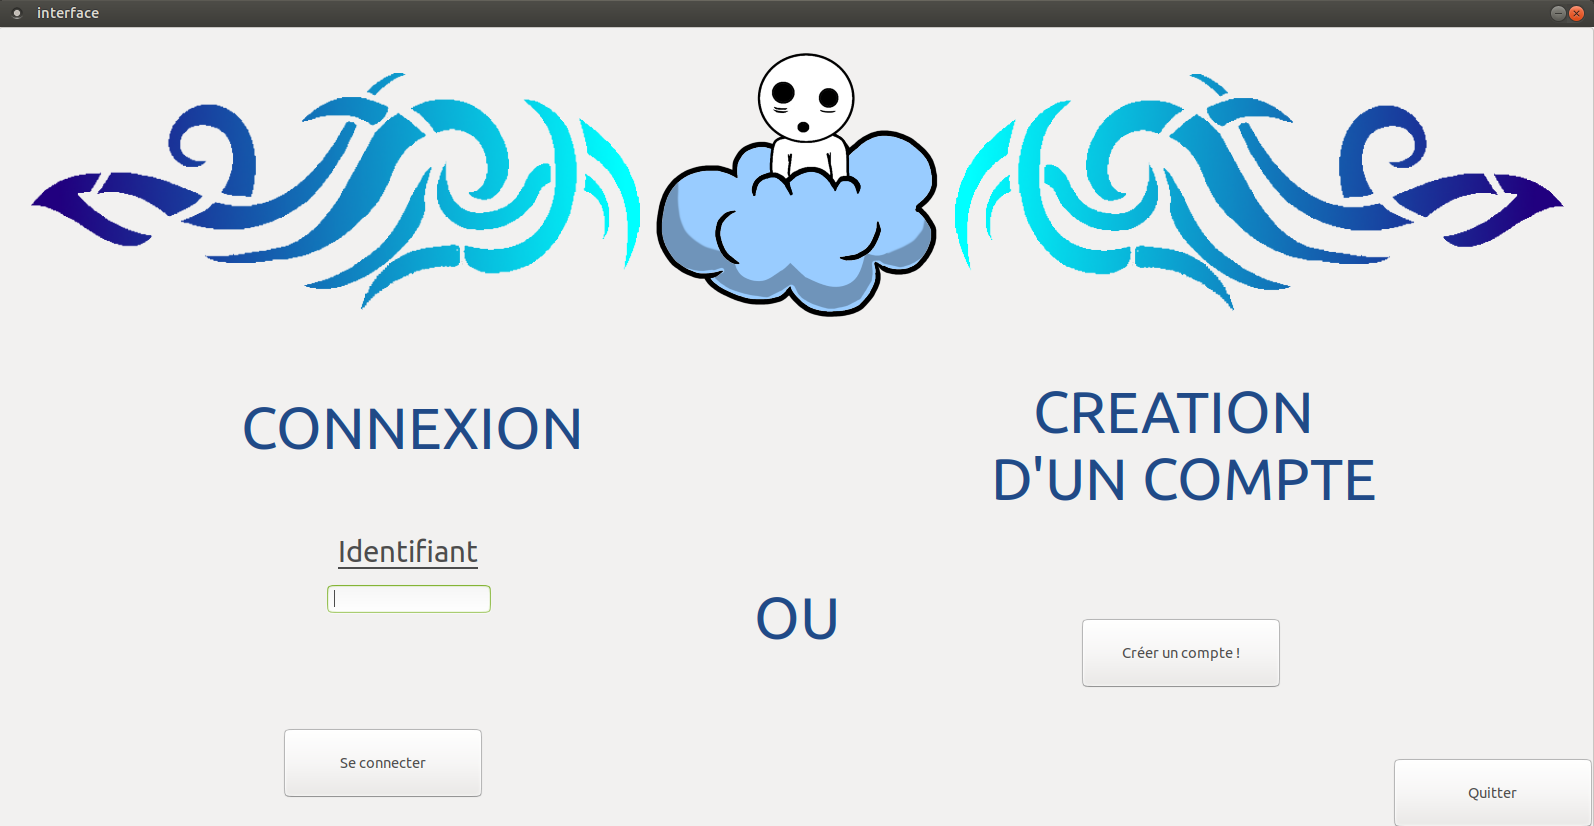
\includegraphics[scale=0.3]{Images/interface1.png}
    \caption{\label{1} Page de connexion}
\end{figure}

\begin{figure}[H]
    \centering
    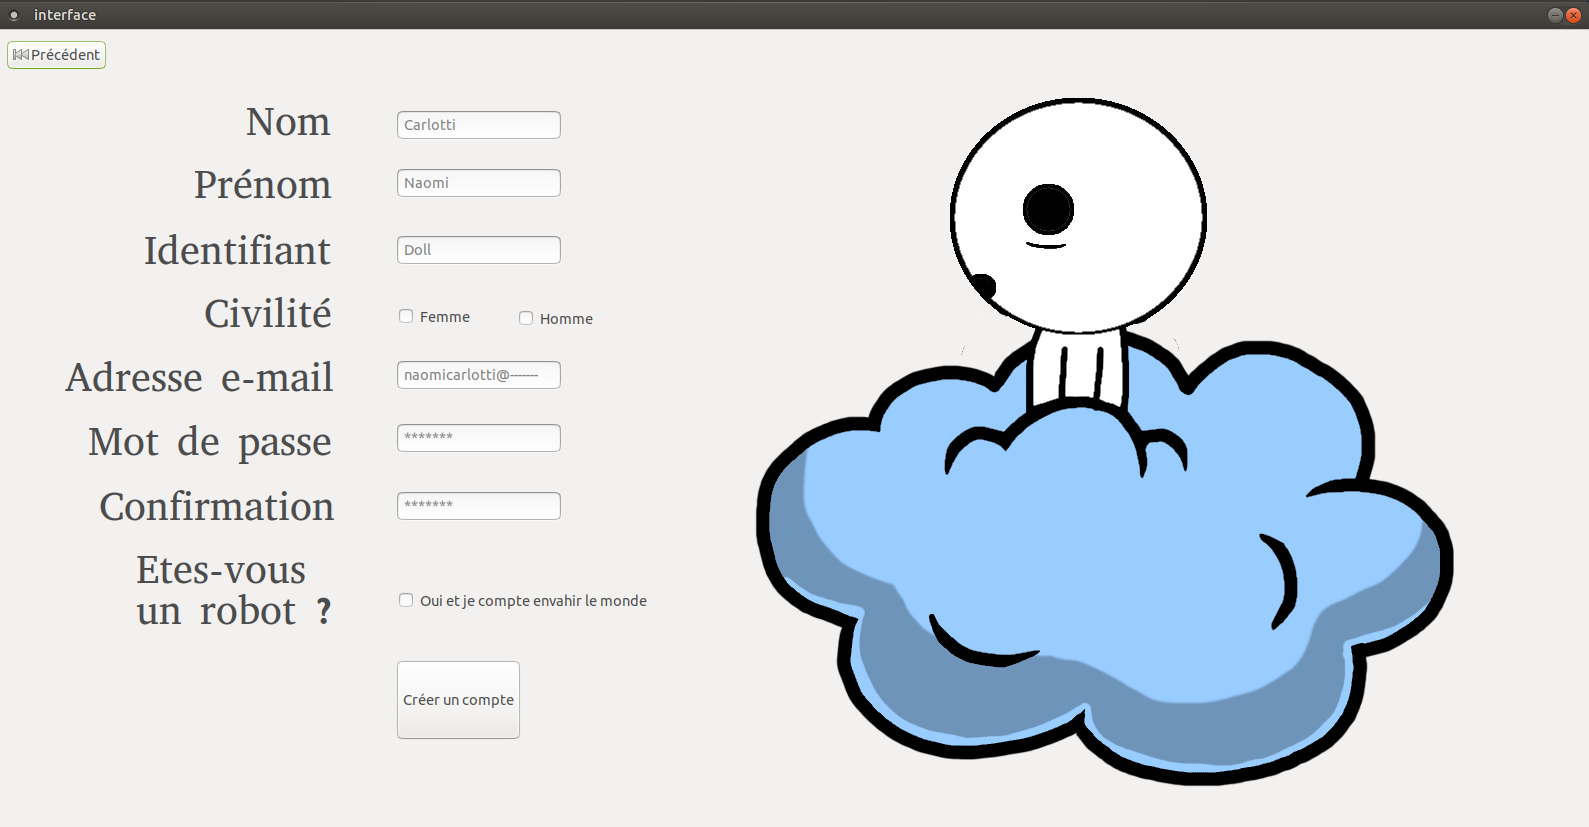
\includegraphics[scale=0.3]{Images/interface5.png}
    \caption{\label{5} Page nouveau compte}
\end{figure}

\paragraph{Page de recommandation}
La page de recommandation est aussi la page d'accueil une fois que l'utilisateur est connecté. Il peut ainsi directement apprécier le contenu que le programme lui propose. De plus, l'utilisateur peut accéder rapidement aux fiches des films proposés.

\begin{figure}[H]
    \centering
    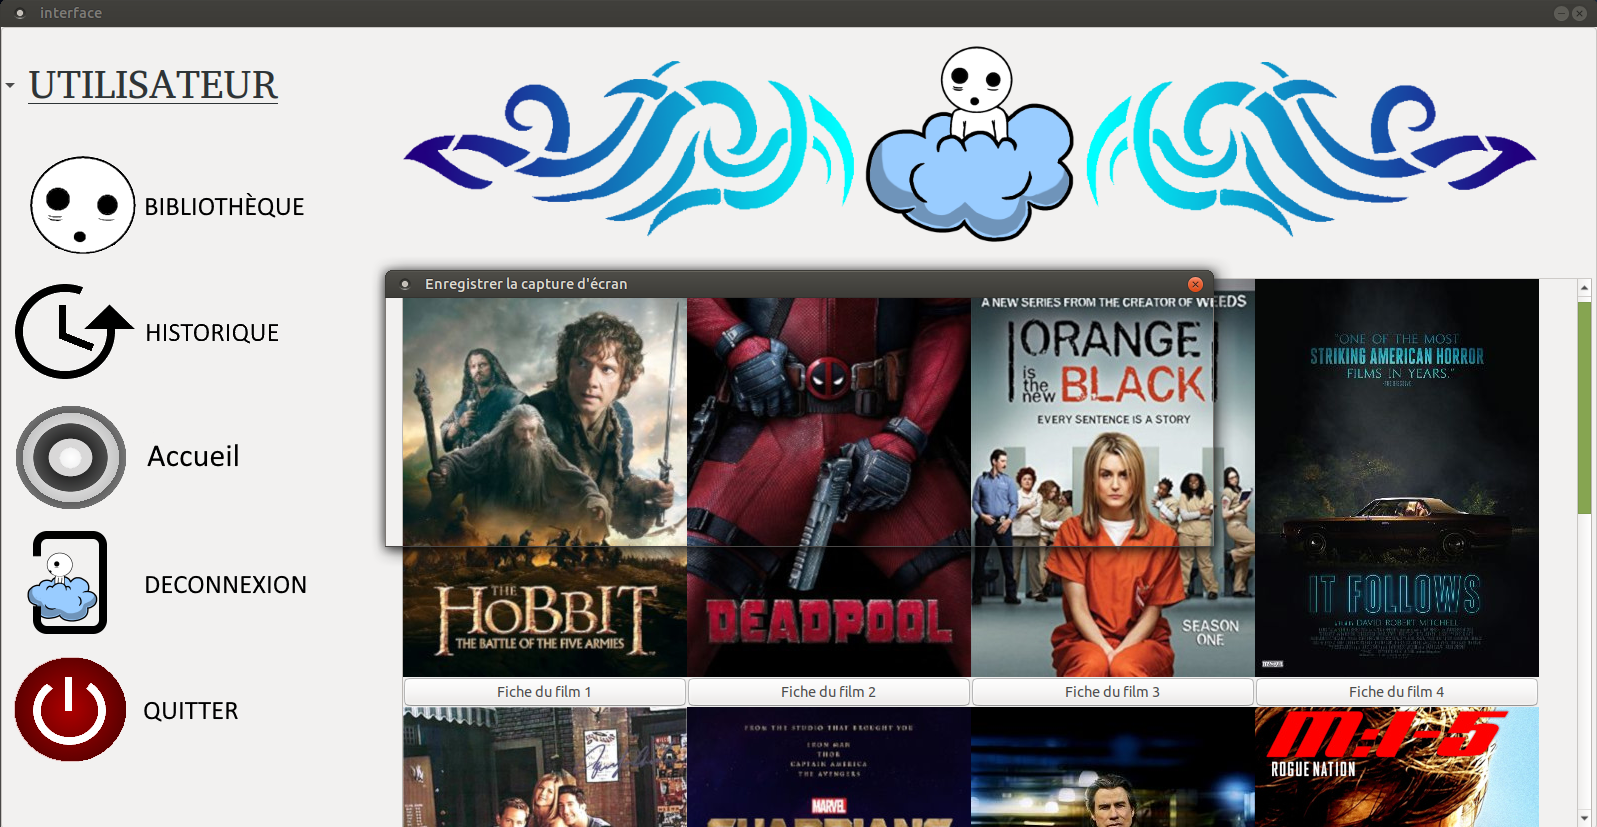
\includegraphics[scale=0.3]{Images/interface2.png}
    \caption{\label{2} Page de recommendation}
\end{figure}

\paragraph{Bibliothèque}
La bibliothèque est accessible via le menu déroulant situé à gauche de l'interface. Elle présente la liste complète des films que référence la base de donnée.\\

Lors de sa réalisation, une question importante s'est posée. Afin d'afficher 100 films, nous pouvions utiliser un tableau, facilement implémentable de manière itérative, ou créer plusieurs image sur la fenêtre bibliothque. Si la première solution permettait un code plus élégant, la seconde offrait une bien meilleure esthétique. En se basant sur les attentes  d'une interface, définie précédemment, nous avons opté pour la seconde solution. Il est à noter que le fait de copier/coller les fonctions répétitives à toutes les images a permis que cette implémentation ne nous soit pas chronophage.

\begin{figure}[H]
    \centering
    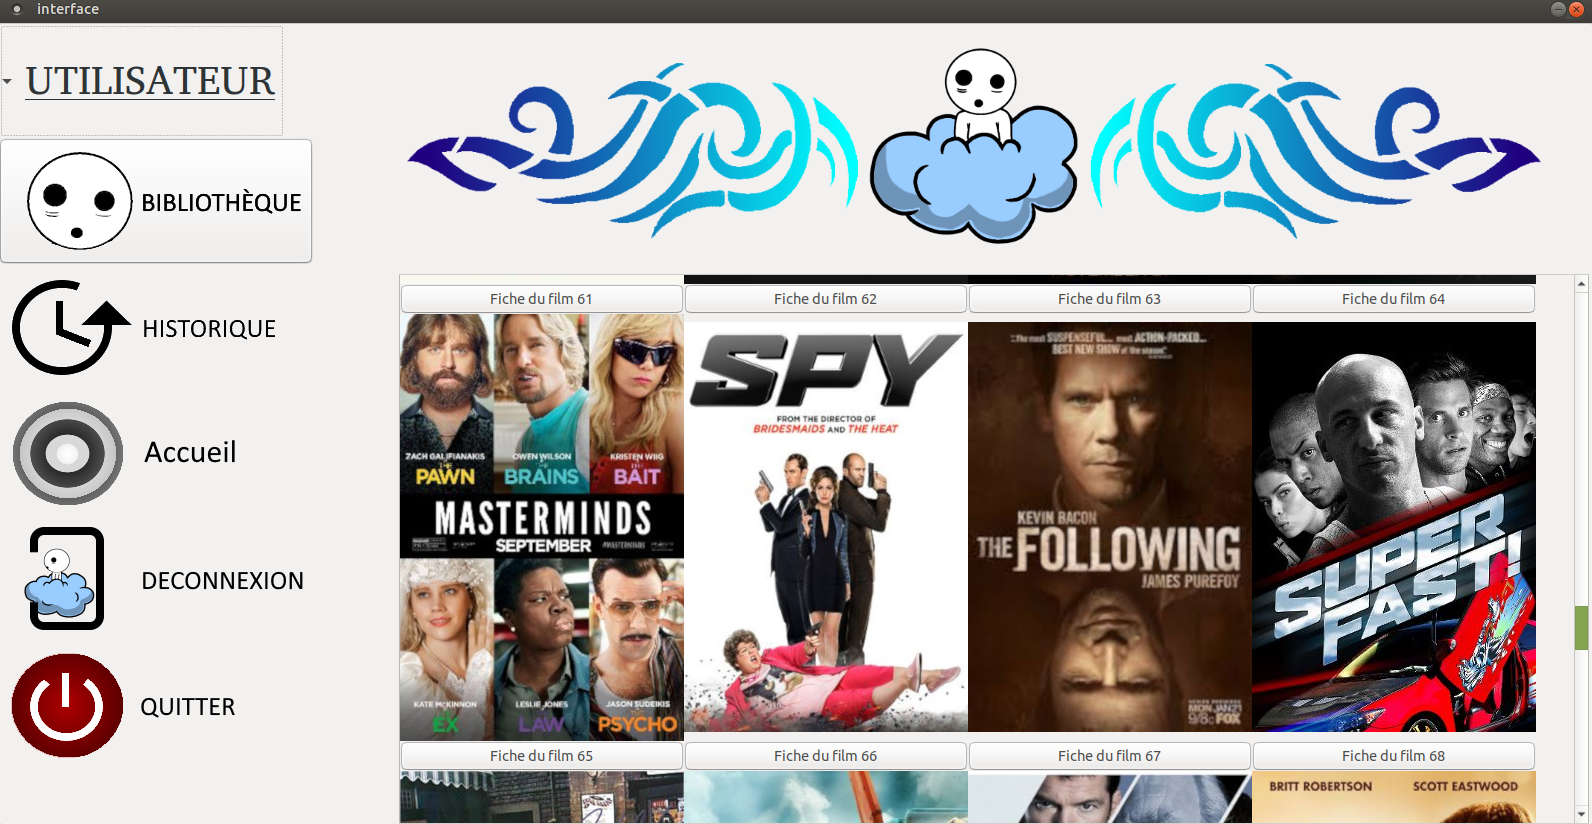
\includegraphics[scale=0.3]{Images/interface3.png}
    \caption{\label{3} Bibliothèque}
\end{figure}

\paragraph{Fiche du film}

Que dire de plus si ce n'est que cette fenêtre permet d'accéder à tous les éléments relatifs à un même film. L'utilisateur peut noter ces derniers à l'aide des nuages qui, en plus d'être intuitifs, s'allient parfaitement avec la charte graphique.

\begin{figure}[H]
    \centering
    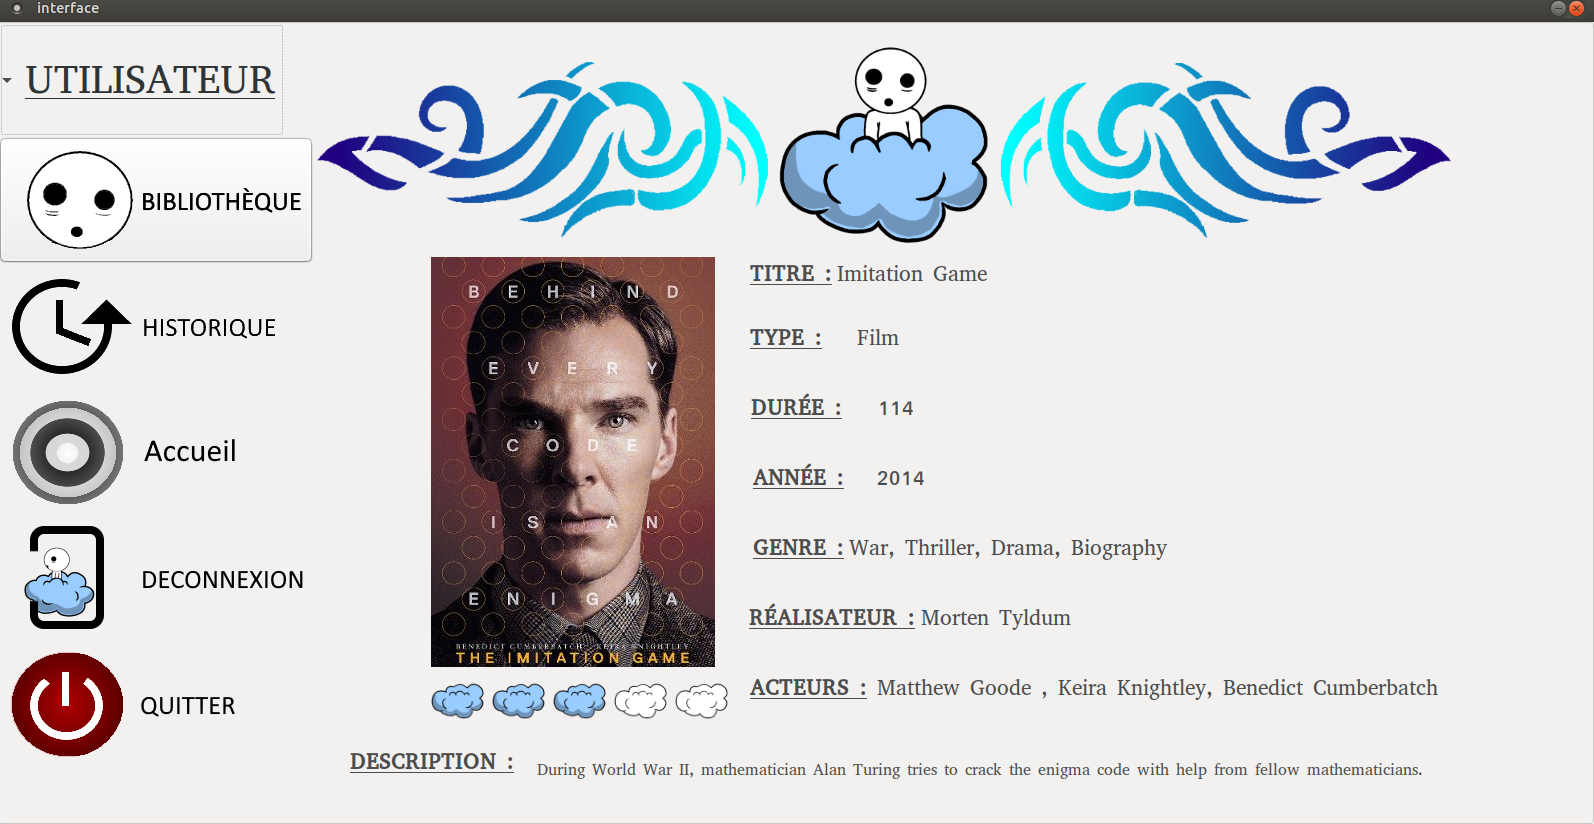
\includegraphics[scale=0.3]{Images/interface4.png}
    \caption{\label{4} Fiche de film}
\end{figure}

\section{Conclusion}

Le groupe dispose de deux interfaces qui recommandent des films ainsi qu'un programme de recommandation. Bien que ces interfaces peuvent être recommandées, elles sont efficientes dans ce qu'elles font. Dans l'ensemble le groupe est satisfait de son travail.

\section*{Annexes}
\addcontentsline{toc}{section}{Annexes}

\subsection*{Sources}

\bibliographystyle{unsrt}
\bibliography{biblio.bib}

\end{document}